%% This file is modified by Jussi Kangasharju and Pirjo Moen.
%% Earlier versions were made by Veli Mäkinen
%% from HY_fysiikka_LuKtemplate.tex authored by Roope Halonen ja
%% Tomi Vainio. Some text is also inherited from engl_malli.tex by
%% Kutvonen, Erkiö, Mäkelä, Verkamo, Kurhila, and Nykänen.
%% 
%% 
% STEP 1: Choose oneside or twoside
\documentclass[english,oneside,openright]{UH_DS_report}
%finnish,swedish
%
%\usepackage[utf8]{inputenc} 
% For UTF8 support. Use UTF8 when saving your file.
\usepackage{lmodern} % Font package 
\usepackage{textcomp} % Package for special symbols 
\usepackage[pdftex]{color, graphicx} % For pdf output and jpg/png graphics 
\usepackage[pdftex, plainpages=false]{hyperref} % For hyperlinks and pdf metadata 
\usepackage{fancyhdr} % For nicer page headers 
\usepackage{tikz} % For making vector graphics (hard to learn but powerful)
%\usepackage{wrapfig} % For nice text-wrapping figures (use at own discretion)
\usepackage{amsmath, amssymb} % For better math
%\usepackage[square]{natbib} % For bibliography
\usepackage[footnotesize,bf]{caption} % For more control over figure captions 
\usepackage{blindtext} 
\usepackage{titlesec}
\usepackage[titletoc]{appendix}
\usepackage{physics}
\usepackage{listings}
\usepackage{graphicx}
\usepackage{subfig}
\graphicspath{ {./images/} }
\onehalfspacing %line spacing
%\singlespacing 
%\doublespacing

%\fussy 
\sloppy % sloppy and fussy commands can be used to avoid overlong text lines

% STEP 2: 
% Set up all the information for the title page and the abstract form. 
% Replace parameters with your information.
\title{Quantum computing and Grover's algorithm} 
\author{Aleksi Suuronen}
\date{\today}
%\prof{Professor X or Dr. Y} 
%\censors{Professor A}{Dr. B}{}
\keywords{Grover's algorithm, Quantum computing, Quantum database search} 
\depositeplace{}
\additionalinformation{}


\classification{\protect{\ \\
    \  Hardware $\rightarrow$ Emerging technologies $\rightarrow$ Quantum technologies $\rightarrow$ Quantum computation\  \\
    \  Theory of computation $\rightarrow$ Design and analysis of algorithms $\rightarrow$ Data structures design and analysis $\rightarrow$ Sorting and searching\\
}}

% if you want to quote someone special. You can comment this line and
% there will be nothing on the document.
%\quoting{Bachelor's degrees make pretty good placemats if you get them
%laminated.}{Jeph Jacques}

% OPTIONAL STEP: Set up properties and metadata for the pdf file that
% pdfLaTeX makes. But you don't really need to do this unless you want
% to.
\hypersetup{ 
	%bookmarks=true,         % show bookmarks bar first?
	unicode=true,           % to show non-Latin characters in Acrobat’s bookmarks 
	pdftoolbar=true,        % show Acrobat’s toolbar?
	pdfmenubar=true,        % show Acrobat’s menu? 
	pdffitwindow=false,		% window fit to page when opened 
	pdfstartview={FitH},    % fits the width of the page to the window 
	pdftitle={},            % title
	pdfauthor={},           % author 
	pdfsubject={},          % subject of the document 
	pdfcreator={},          % creator of the document
	pdfproducer={pdfLaTeX}, % producer of the document
	pdfkeywords={something} {something else}, % list of keywords for
	pdfnewwindow=true,      % links in new window 
	colorlinks=true, 		% false: boxed links; true: colored links 
	linkcolor=black,        % color of internal links 
	citecolor=black,        % color of links to bibliography 
	filecolor=magenta,      % color of file links 
	urlcolor=cyan			% color of external links
}
          
\begin{document}

% Generate title page.
\maketitle

% STEP 3: Write your abstract (of course you really do this last). You
% can make several abstract pages (if you want it in different
% languages), but you should also then redefine some of the above
% parameters in the proper language as well, in between the abstract
% definitions.

\begin{abstract} 
% Use one or two paragraphs to summarize the main contributions of your report. Some example sentences
% are like: "I have read five papers [1-5] on graph data management in this seminar. In this report, I review their
% main contributions on the problem of big graph processing."

Grover's algorithm is a quantum algorithm, which can be used for searching unstructured databases quadratically faster on a quantum computer, than existing searching algorithms on classical computers. Quantum algorithms are ran on quantum computers, which use a computing paradigm called quantum computing. Quantum computing takes advantage of quantum mechanical effects, such as quantum parallelism. This results in more computing power for certain computational problems, like integer factorization and database querying.

For this report, I have read 9 papers [1 -- 9] about quantum search algorithms, such as Grover's algorithm, and about quantum computing and its relation to databases. During this report, I will tell about Grover's algorithm and also provide an introduction to the field of quantum computing. Furthermore, I have read a paper and done research on the internet, how to program quantum algorithms using an open-source framework for Python called Qiskit, and how to deploy and run them on a real quantum computer. In this report, I will compare running Grover's algorithm on IBM's cloud services on a quantum computer simulator versus on a real quantum computer on the same searching related task.

\end{abstract}

% Place ToC
\mytableofcontents

\mynomenclature

% ----------------------------------------------------------------------
% STEP 4: Write the report. Your actual text starts here.
% You shouldn't mess with the code above the line except to change the
% parameters. Removing the abstract and ToC commands will mess up stuff.

\chapter{Introduction}
\label{chapter:intro}
%Give the motivation of the research problem and discuss the main results of previous papers. The length of Introduction is around 1 - 1.5 pages. At the end of the Introduction, give the organization of the rest of the report. An example is like: "The rest of the report will be divided as follows. In Section 2, I will discuss how big data applies to health by providing explanations. Then, in Section 3, I will give an overview of the potential areas.. Finally, I will give a brief conclusion to summarize this report."

Quantum computing is an emerging technology and computing paradigm, which combines quantum mechanics and computer science \cite{ambainis2004quantum, qcdb}. Richard Feynman was the first one to introduce the idea of quantum computing in the 1980's, by observing that quantum mechanical effects could not been efficiently simulated on a classical computer \cite{introtoqc}. At first the scientific community were not interested in the field of quantum computing, as building quantum computers turned out to be difficult and there were no scientific proof that quantum computers would be much more faster and efficient than classical computers. 

However, in 1994, Peter Shor introduced a quantum algorithm for efficient integer factorization called Shor's algorithm \cite{introtoqc}. Shor's algorithm proved to run in polynomial time, when existing factorization algorithms ran in exponential time. This resulted in quantum computing gaining more interest. In 1996, Lov K. Grover introduced a quantum algorithm called Grover's algorithm for searching unstructured databases quadratically faster than known classical algorithms \cite{grover1996fast}. These two quantum algorithms are the most groundbreaking algorithms in the field of quantum computing, as they were the first ones proven to be faster on a quantum computer than existing algorithms on a classical computer \cite{ambainis2004quantum}. Both have also real world applications, for example in the field of cryptography with disruptive results.

This report focuses on Grover's algorithm. The rest of the report will be divided as follows. In Section 2, related work is discussed. I will give both a summary and explanation about Grover's algorithm, how it has been researched in the past and what are the application areas of it. I will also discuss about the state of the research combining quantum computing and databases. In Section 3, I will give a more detailed explanation about quantum computing and Grover's algorithm. In Section 4, I will discuss about the weak points I have found in the picked papers. In Section 5, I will present experiments regarding Grover's algorithm by using Qiskit, an open-source programming framework for quantum computing. I will run Grover's algorithm on a real quantum computer through IBM's cloud services and on a quantum computer simulator, and compare and analyze the results. Finally in Section 6, I will give a brief conclusion to summarize this report.

\chapter{Related work}
\label{chapter:relatedwork}
%This part makes a literature review on the particular topic defined in the Introduction. This part is both a summary and explanation of the complete and current state of knowledge on the topic. It provides a constructive analysis of the methodologies and approaches of other researchers. The length of this part is around 1.5 -- 2 pages.

In this Chapter, I will present the history of Grover's algorithm, how it has been researched and what are its applications outside of databases and data management.

%\section{Quantum computing}

%The concept of quantum computing and quantum computers arose in the 1980's, proposed by Richard Feynman \cite{introtoqc}. The scientific community did not show much particular interest to the field back then, as there were no knowledge of how to build these machines, or how much more powerful they would be in certain problems compared to classical computers. In 1994, Peter Shor developed Shor's algorithm, which is a quantum algorithm for factoring large integers in polynomial time using a quantum computer, when the best known algorithm for factoring large integers on a classical computer has exponential time complexity. Factoring large integers with a classical computer is a NP--hard problem, to which multiple modern day cryptographic techniques rely on and what Shor's algorithm jeopardises. This led scientists and researchers to study and develop quantum computing, and later post-quantum cryptography \cite{introtoqc, qcdb}.

\section{Data searching}

Following the founding of Shor's algorithm, Grover's algorithm was first introduced by its creator Lov K. Grover in 1996 \cite{grover1996fast}. Grover's algorithm is a quantum algorithm, which provides a quadratical speed-up for searching an unsorted database. Assume we have a database, which has $N$ elements, and we want to find one exact element without knowing anything about the database and its structure. With a classical computer the best running time algorithm to find the element would need on average $O(N)$ queries. On a quantum computer, Grover's algorithm would find the wanted element in $O(\sqrt{N})$ quantum queries. Grover's algorithm has been proven to be the fastest algorithm for searching an unsorted database \cite{giri2017review, introtoqc} and has been under extensive research in the field \cite{giri2017review}.

Grover's algorithm can be used both for searching a single entry or multiple entries from an unsorted database \cite{giri2017review}. The optimal amount needed for finding $M$ entries from a $N$--sized database is $\frac{\pi}{4}\sqrt{\frac{N}{M}} = O(\sqrt{\frac{N}{M}})$ quantum queries. Grover's algorithm does not only limit to a full database search, as it can be also used for a partial database search for efficiency reasons. However, it is case by case when this partial database search is more efficient than a full database search. This partial search algorithm is proven to need $(\frac{\pi}{4}+\frac{\beta (K) - \eta (K)}{\sqrt{K}})\sqrt{N}$ quantum queries. However, there is also an optimized version of this partial search algorithm, which is obtained by optimizing the coefficient $\beta (K) - \eta (K)$.

Other than using Grover's algorithm for quantum database search, there is not much of research or literature about combining quantum computing and data management \cite{qcdb}. Quantum computing has some applications in the field of optimizing database queries, but it will not be discussed further in this report.

\section{Cryptanalysis}

Both Shor's algorithm and Grover's algorithm can be used in the field of cryptanalysis \cite{grassl2016applying}. In theory, Shor's algorithm can be used for decrypting the encryption keys used in asymmetric\footnote{Also known as public-key encryption.} encryption through efficient integer factorization. In reality, this would need a big enough and functioning quantum computer to be considered as a threat. Meanwhile, Grover's algorithm can be used for decrypting the encryption keys used in symmetric cryptography. In this case we are especially talking about the Advanced Encryption Standard (AES) scheme. Grover's algorithm can be used to gain quadratic speed-up in brute-force attacks related to exhaustive key search in AES. Exhaustive key search means that every possible solution for the encryption key is tried one at a time to decrypt the encryption key.

\section{NP-complete problems}
Grover's algorithm can also be applied to some NP-complete problems, like \emph{3-SAT}\footnote{Also known as boolean 3-satisfiability} \cite{ambainis2004quantum} and \emph{graph-coloring} \cite{introtoqc}, as they can be modeled as search problems. The satisfiability problem can be described in the following way:

Let $F$ be a boolean formula in the form of $F(x_{1}, \ldots, x_{N})$. Does one of $2^{n}$ assignments to $x = (x_{1}, \ldots, x_{n})$ of values to the variables make $F$ true?

The problem resemblances the previously mentioned exhaustive key search. The brute-force exhaustive search needs to test $2^{n}$ assignments to solve the problem. However, using a quantum computer, Grover's algorithm needs to test $O(\sqrt{N}) = O(1.41..^{n})$ assignments to solve the problem.

\chapter{Detailed methods and ideas in previous works}
\label{chapter:previouswork}
%This part can be extended to several sections which depend on the number of papers you read and the contents you want to present. Please add more examples and figures to illustrate the results. Do not directly copy the esentences from previous papers. Rephrase the ideas according to your own understanding.

In this Chapter, I will introduce quantum computing in more detail. I'll present how information is handled and presented inside a quantum computer compared to a classical computer, why (in theory) quantum computers are more powerful than classical computers and what are the challenges in quantum computing and building (large-scale) quantum computers. We will also present the functioning of Grover's algorithm in more detail, such as how it finds the right element in the database and other properties.

\section{Quantum Computing in Detail}

\subsection{Quantum information}
In a classical computer, information is described and handled as bits. A single bit can only have a single value of $0$ or $1$ at a time. These bits are then manipulated through different gates, such as \emph{NOT} and \emph{NAND}, and these multiple gates form circuits. However, a quantum computer uses quantum bits, also known as qubits, as its unit of information \cite{introtoqc}. Qubits are usually presented by using the bra/ket-notation\footnote{Sometimes also referred as the Dirac notation} and the classical bit values of $0$ and $1$ can be presented as qubits $\ket{0}$ and $\ket{1}$. What is special about qubits compared to classical bits, is that qubits can be in a linear combination of states $\ket{0}$ and $\ket{1}$ \cite{lavor2003grover}. This state is called a superposition of states $\ket{0}$ and $\ket{1}$, e.g., $x \ket{0} + y \ket{1}$. In this case numbers $x$ and $y$ are complex numbers, also called probability amplitudes, such that $|x|^{2} + |y|^{2} = 1$ \cite{qcdb}. This can be interpreted as measuring the value $\ket{0}$ with the probability of $|x|^{2}$ and value $\ket{1}$ with the probability of $|y|^{2}$. These qubits are then controlled through quantum circuits, which consists of quantum gates \cite{lavor2003grover}. Some examples of one-qubit gates are the \emph{NOT} and \emph{Hadamard} gates.

\subsection{Quantum parallelism}
The interest in quantum computing is due to the fact that quantum effects in quantum systems provide exponential parallelism, called quantum parallelism \cite{introtoqc}. This can then be harnessed to solve certain computational problems faster than with a classical computer. Both Shor's and Grover's algorithms take advantage of this phenomenon, which results in them being so efficient.

 A register of bits in a classical computer can store $2^{n}$ values, where $n$ is the amount of bits, and only one of the values can be present at a time \cite{introtoqc}. However, a register of qubits can be in a superposition of all $2^{n}$ values. This exponential growth of the state space is the reason why quantum computers are believed to be exponentially faster than classical computers. In other words, when a classical computer can produce a single output for one input value, a quantum computer can produce all of the possible outputs for the input in the same time.

On a classical computer, speeding up computations can be achieved through parallelization. Achieving exponential decrease of time used for computation requires an exponential increase in the amount of needed processors and hence, an exponential increase in physical space needed for the processors \cite{introtoqc}. In quantum systems the situation is different, as parallelism increases exponentially in relation to the size of the system. Therefore, exponential increase in parallelism scales linearly in relation to the needed physical space.

\subsection{Challenges in quantum computing}
In quantum computing, there are some trade-offs related to the exponential computing power. When a quantum procedure is run and then the result is read, this disturbs the quantum state by destroying the rest of the quantum states \cite{introtoqc}. Also, as quantum algorithms are probabilistic due to the nature of quantum mechanics, the measured result might not even be the one we are looking for. However, there are some techniques how to increase the probability of getting the right result by modifying quantum states. In the next Section \ref{detailedgrover}, we will inspect how Grover's algorithm does this.

What comes to the implementation of quantum computers, a big challenge is decoherence \cite{introtoqc}. Quantum states are very fragile and prone to distortions coming from the surrounding environment. Therefore, quantum computers need a very isolated environment, so that the quantum states do not interfere with the outside environment, making the computation and measuring reliable. Quantum error correction is a technique used for reconstructing the quantum states without errors.

\section{Grover's Algorithm in Detail}
\label{detailedgrover}

Grover's algorithm can be formally defined as a function \cite{lavor2003grover}
\begin{equation}
    f : \{ 0, \ldots, N - 1 \} \rightarrow \{0, 1\},
\end{equation}
which recognizes:
\begin{equation}    
f(i) = 
\begin{cases}
    1 \textrm{ if $i$ is the searched element,} & \\ 0 \textrm{ otherwise.}
\end{cases}
\end{equation}

Grover's algorithm uses two quantum registers: the first one is used to store $n$ qubits, and the second one is used to store only one qubit \cite{lavor2003grover}. Let $N = 2^{n}$ for some integer $n$, and $U_{f}$ a quantum gate:
\[U_{f} : \ket{x, 0} \rightarrow \ket{x, P(x)},\]
where $P(x)$ is a function, which tells if $x$ makes the statement true by returning 1 \cite{introtoqc}.

The first step of Grover's algorithm is to initialize the first register, which contains the superposition of all possible $2^{n}$ values $x_{i} \in \{\ket{0}, \ldots, \ket{2^{n} - 1}\}$. Hence, we get the register
\begin{equation}
\label{eqn: 1}
    \frac{1}{\sqrt{2^{n}}}\sum_{x = 0}^{n - 1}\ket{x} .
\end{equation}

Now due to quantum parallelism, when $U_{f}$ is applied to the first register, $P$ is computed for all $x_{i}$, which leads to state of the register being in a superposition state
\begin{equation}
\label{eqn: 2}
\frac{1}{\sqrt{2^{n}}}\sum_{x = 0}^{2^{n} - 1}\ket{x, P(x)}.    
\end{equation}

Now any value $x_{0}$, which results in making $P(x_{0})$ true, the quantum state $\ket{x_{0}, 1}$ is included in the superposition. As every quantum state has the amplitude of $\frac{1}{\sqrt{2^{n}}}$, the probability when randomly measured getting $x_0$ is $\frac{1}{2^{n}} = 2^{-n}$, which is significantly small. The technique here is to modify the quantum state in \ref{eqn: 2} so that the amplitude of vectors $\ket{x_{0}, 1}$, which make $P$ true is significantly higher, than the amplitude of vectors $\ket{x, 0}$, which make $P$ false. The computing of $P(x_{i})$ and changing the amplitude is then iterated $\frac{\pi}{4} \sqrt{2^{n}}$ times, and then the result is obtained by measuring the last qubit. Therefore, as a result of the amplitude change, it has a high probability of being $1$. This technique of changing the amplitude of the states, which have the desired result is called Amplitude Amplification and is a common technique when working with quantum algorithms \cite{lavor2003grover}. I will not present Amplitude Amplification on any deeper level, however image \ref{groverflow} shows the flow of the Grover's algorithm, as presented in \cite{zhang2020recent}.

It has also been researched that Grover's algorithm is efficient only to a certain factor \cite{introtoqc}. The most optimal factor is $\frac{\pi}{4}$, which provides a failure rate of $2^{-n}$. More iterations grow the failure rate, and after $\frac{\pi}{2}\sqrt{2^{n}}$ iterations the failure rate is almost 1. This behaviour differs from classical algorithms, where more iterations usually provide better results. When iterating quantum procedures, the results get better only up to a certain point, and after that they will get worse again. So to get useful results, it is important to know when to stop the iterating.

\begin{figure}[h]
\caption{Flow of the Grover's algorithm}
\label{groverflow}
\centering
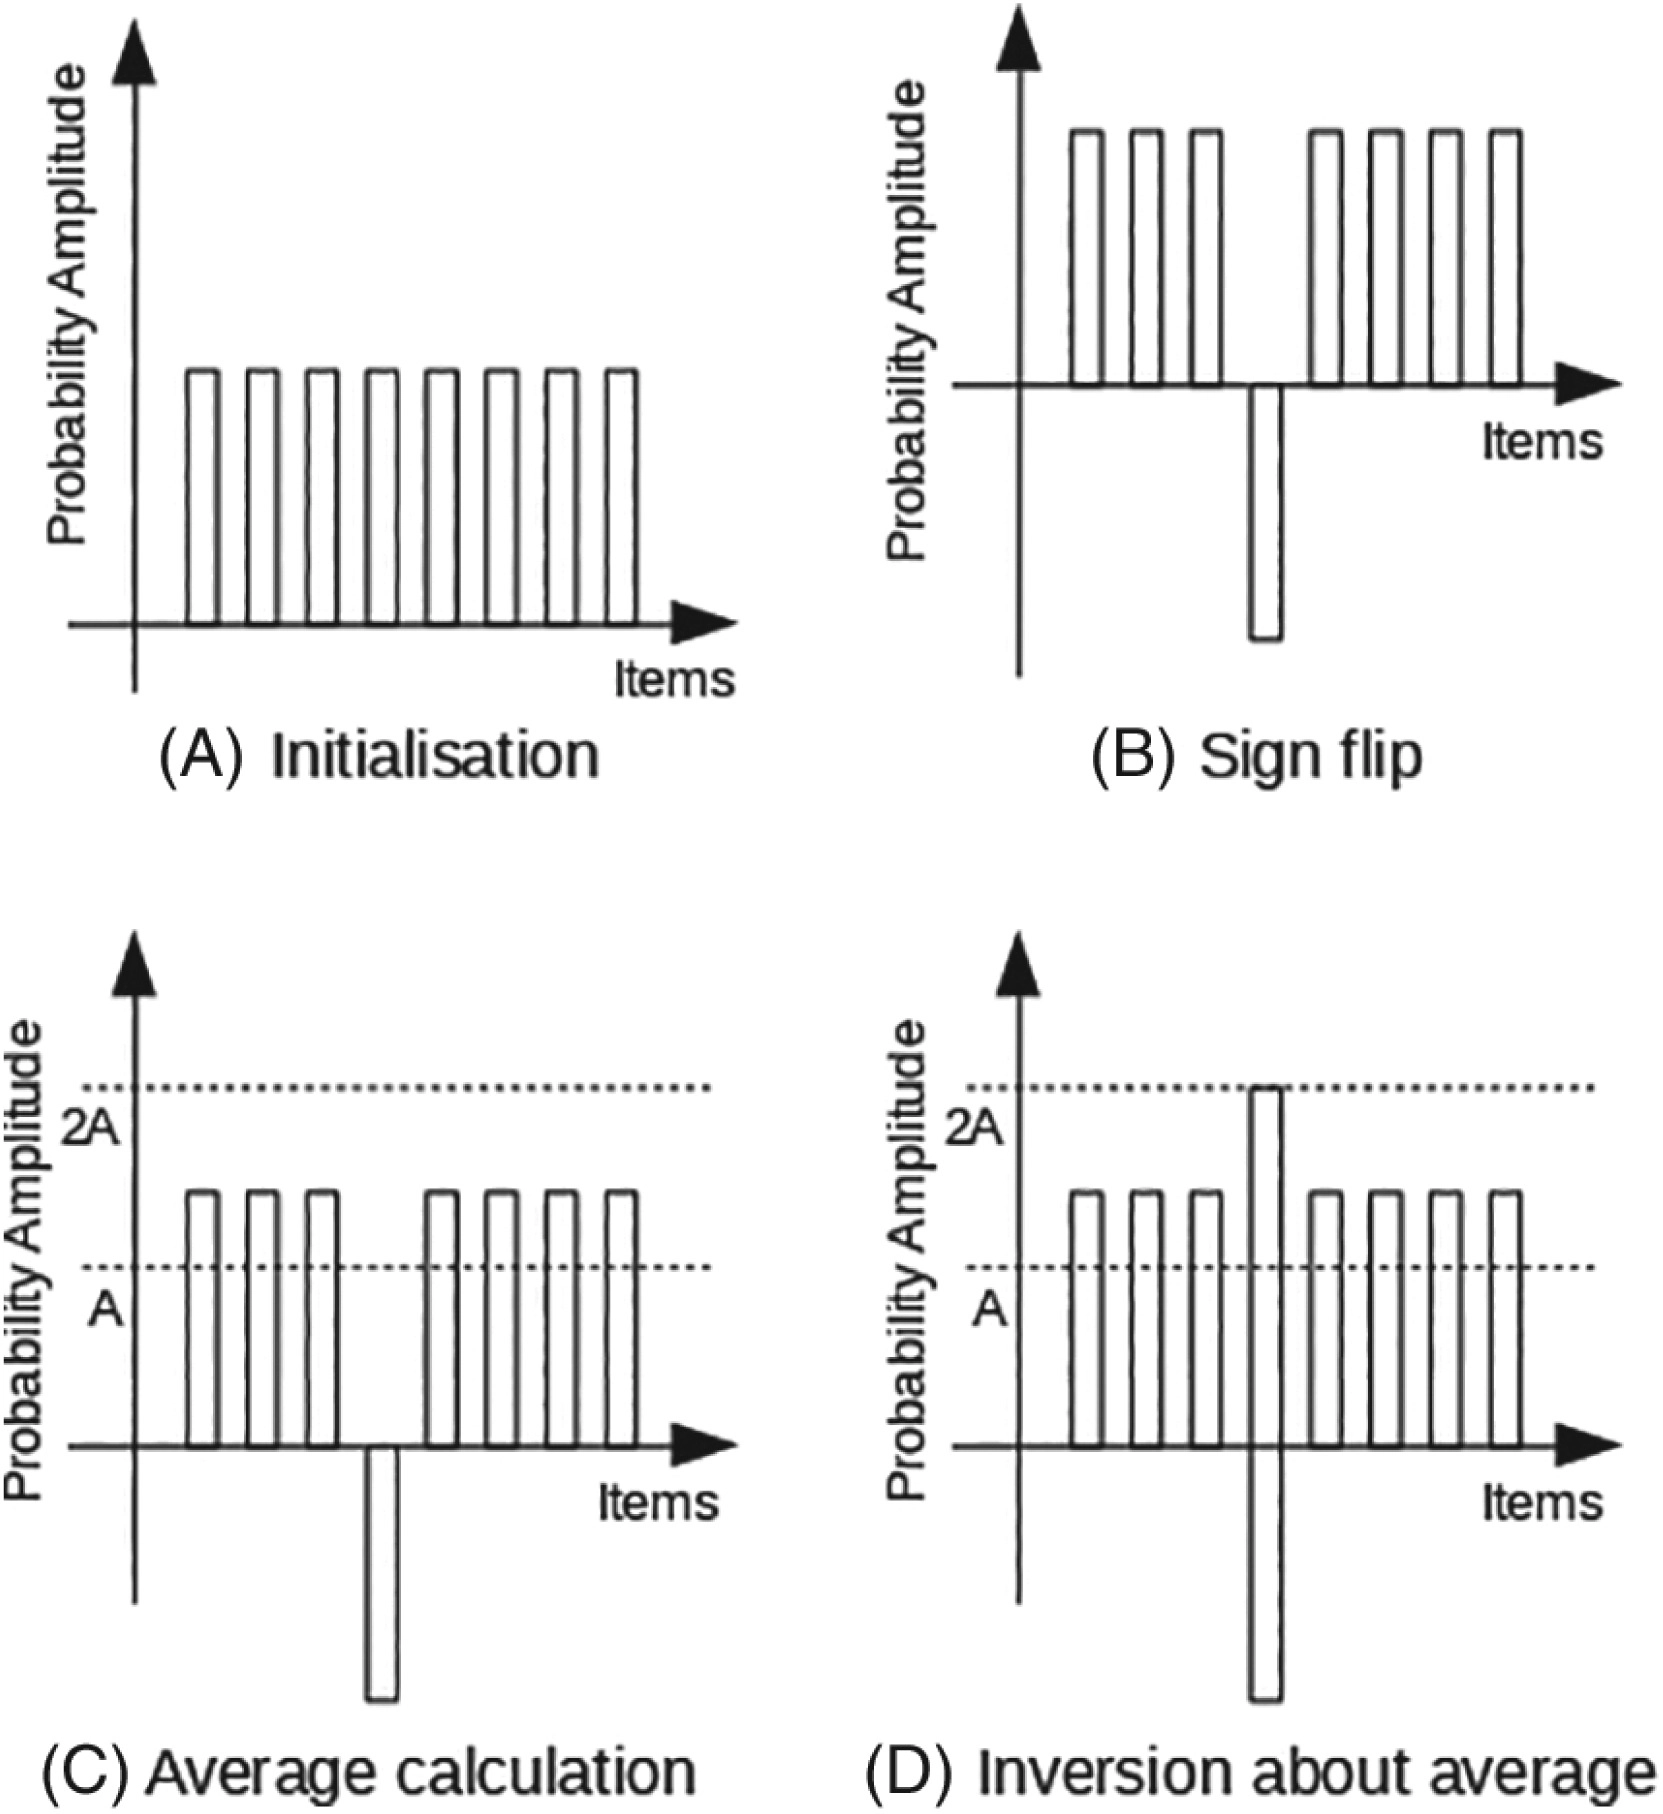
\includegraphics[width=\linewidth]{images/grover-flow.png}
\end{figure}

\chapter{Weak points of papers and open challenges}
\label{chapter:weakpoints}
%Several weak points of papers are found and explained in this section. The legnth is around 0.5 -- 1 pages. Some examples are like "The main weak point I figured out is that there is no enough explanation on...", "The concept is not well defined and it is confused for readers.".

I found a few weak points in the papers used in this report. The main weak point, which I noticed is that the research on quantum computing and quantum algorithms is mostly theoretical. The papers do not present any empirical benchmarking or exact numbers what comes to the power of quantum computing and efficiency of quantum algorithms compared to classical computers. It would be interesting to see comparison between classical and quantum computers, for example in the amount of needed qubits, memory, time or energy efficiency for a computing task.

However, I think there are multiple reasons for the lack of exact benchmarks. First of all, quantum computing is a fairly new topic and some of the papers used for this report are fairly old. Also as mentioned in \cite{qcdb}, there is not a lot of research, which combines databases and quantum computers. Second of all, quantum computing might be a discipline, which develops faster than what the scientific articles get published. As working quantum computers have groundbreaking consequenses in the field of cryptography, it might be that some of the research is kept under the radar on purpose.

Maybe one of the greatest open challenges is how powerful quantum computers can be realistically built and what they are capable of computing better than classical computers. One challenge is also to find an algorithm, which would give a greater speed-up than the Grover's quadratical one.

\chapter{Ideas, algorithms and experiments}
\label{chapter:ideas}
%Give new ideas/algorithms/experiments on this research problem. This part is very important, because it shows the potential of the author to be an independent innovative researcher. This section can be as long as possible.

In this Chapter, I will describe and explain the experiment setup and the experiments related to Grover's algorithm. The experiment is quite trivial, but enough how to demonstrate the functioning of Grover's algorithm in a search related problem. The same task will be run on IBM's cloud services on a quantum computer simulator and on a real quantum computer, after which the results are analyzed.

\section{Problem and Experiment Setup}
Qiskit is an open-source framework backed by a company called IBM, which can be used for coding quantum algorithms using Python without needing a broad background in quantum physics \cite{https://doi.org/10.48550/arxiv.1903.04359}. With Qiskit you can run your quantum algorithms on a simulator or on a real quantum computer through multiple providers, such as IBM or Amazon Web Services. In this report, Grover's algorithm is run on both situations, on a simulator and on a real quantum computer through IBM's cloud services. IBM was chosen as a provider due to extensive documentation and compatibility, as Qiskit is maintained by IBM.

For the experiment, a quantum computer called \emph{ibm\_oslo} was used. It was chosen due to being free of charge to use, and due to geographical location to minimize latency. However, as it can be used free of charge, this is shown as long queues to get your job running on the system. Also it has a lower quantum volume and less qubits than the ones included in the paid premium plan. More precisely, \emph{ibm\_oslo} has Falcon r5.11H processor, $7$ qubits of computing power, quantum volume of 32 and can do around 2600 circuit layer operations per second (CLOPS).

For the simulations, the used simulator is called \emph{QASM}. \emph{QASM} is a general-purpose simulator for simulating quantum circuits ideally and subject to noise modeling, while supporting 32 qubit computations.

The problem used here is quite simple, but is enough to demonstrate the idea and functioning of the Grover's algorithm. Let there be an array, which will have 8 entries $[0, \ldots, 7]$, from which a random value will be picked. In this experiment the value to be found was $0$ or $\ket{000}$. The random value is then given to an \emph{oracle}, which is a black box telling if the guessed entry is correct or not. After that Grover's algorithm is used to find the correct element, which is the one that has the highest probability. As $2^{3}=8$, $3$ qubits is needed for the computation. Grover's algorithms is also iterated different amount of times to see how this affects to the results and probabilities. Visualization is done by using Python and matplotlib library. The graphs are also available through IBM's cloud services, and they are available for viewing in GitHub, see Appendix \ref{appendix:testdataresults}. The whole program code can be found from behind the link in Appendix \ref{appendix:code}.

\section{Results of the experiments}
\label{Allresults}

\subsection{Simulator}
\label{simulator}
\begin{figure}[h]
\caption{Results and visualization given by the simulator}
\centering
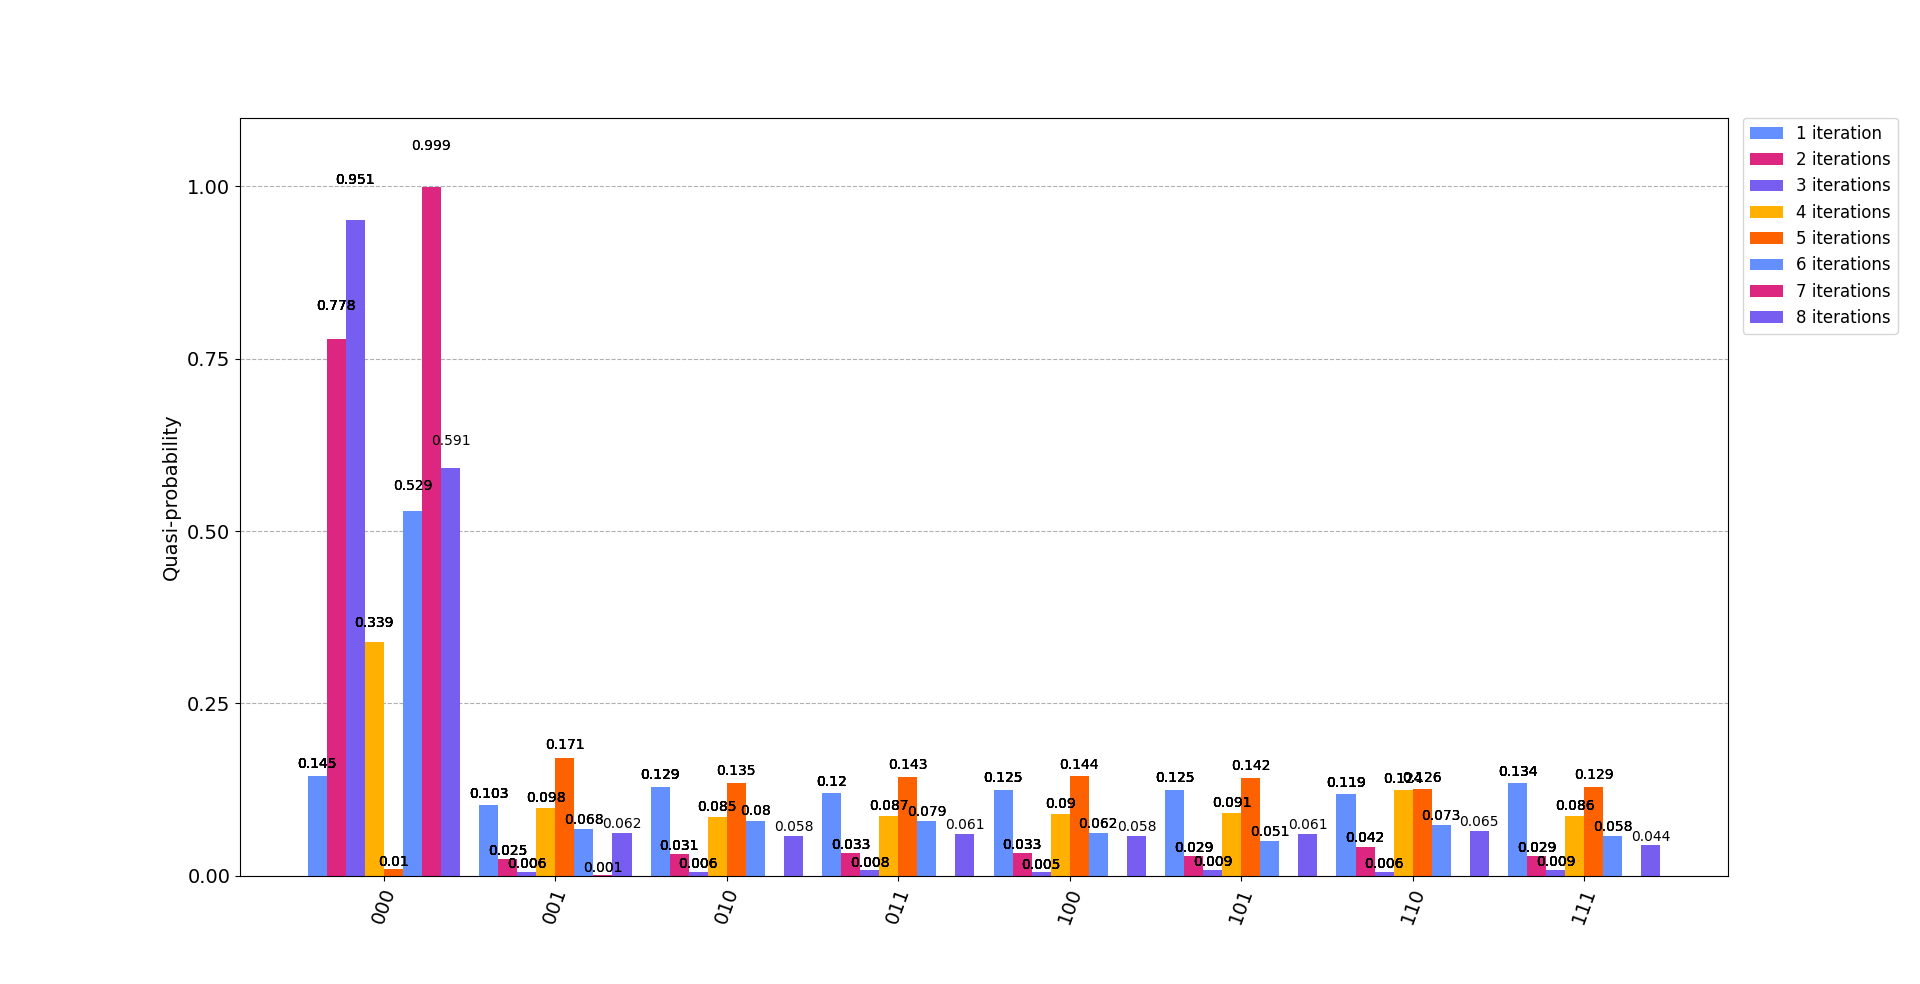
\includegraphics[width=\linewidth]{images/simulator/Figure_1.png}
\end{figure}

The different colors of the bars indicate on how many iterations the Grover's search algorithm is run. The y-axis is the probability of getting a certain entry with a certain amount of iterations, and this probability can also be read from the top of the bars in the bar chart. The x-axis represents the entries in the database, in this case the values $[0,\ldots,7]$, which can be encoded as qubits $\ket{000}, \ket{001}, \ket{010}, \ket{011}, \ket{100}, \ket{101}, \ket{110} \text{and} \ket{111}$.

For example, the bar chart above shows that with $1$ iteration, the probability of getting $\ket{000}$ is $0.145$, $\ket{001}$ is $0.103$ and so on. The probabilities, which are higher on the other values than on $\ket{000}$, are therefore wrong. So it can be seen that the simulator found the correct entry on all, but the $5$ iterations. In \ref{detailedgrover} it was stated that the optimal amount of iterations is $\frac{\pi}{4} \sqrt{2^{n}} = \frac{\pi}{4} \sqrt{8} = 2.22 $. However, it seems that with $3$ iterations we get the largest probability of $0.951$. For some reason, with 7 iterations, the probability is almost $1$, but it has not computed any probabilites for other values. This behaviour could be investigated more, as it is not clear if this is some programming error in my code or in the framework, or is this just natural behaviour of the algorithm.

 More detailed results of this test run can be found from Appendix \ref{appendix:testdataresults}.

\subsection{Real quantum computer}

\begin{figure}[h]
\caption{Results and visualization given by the real hardware}
\centering
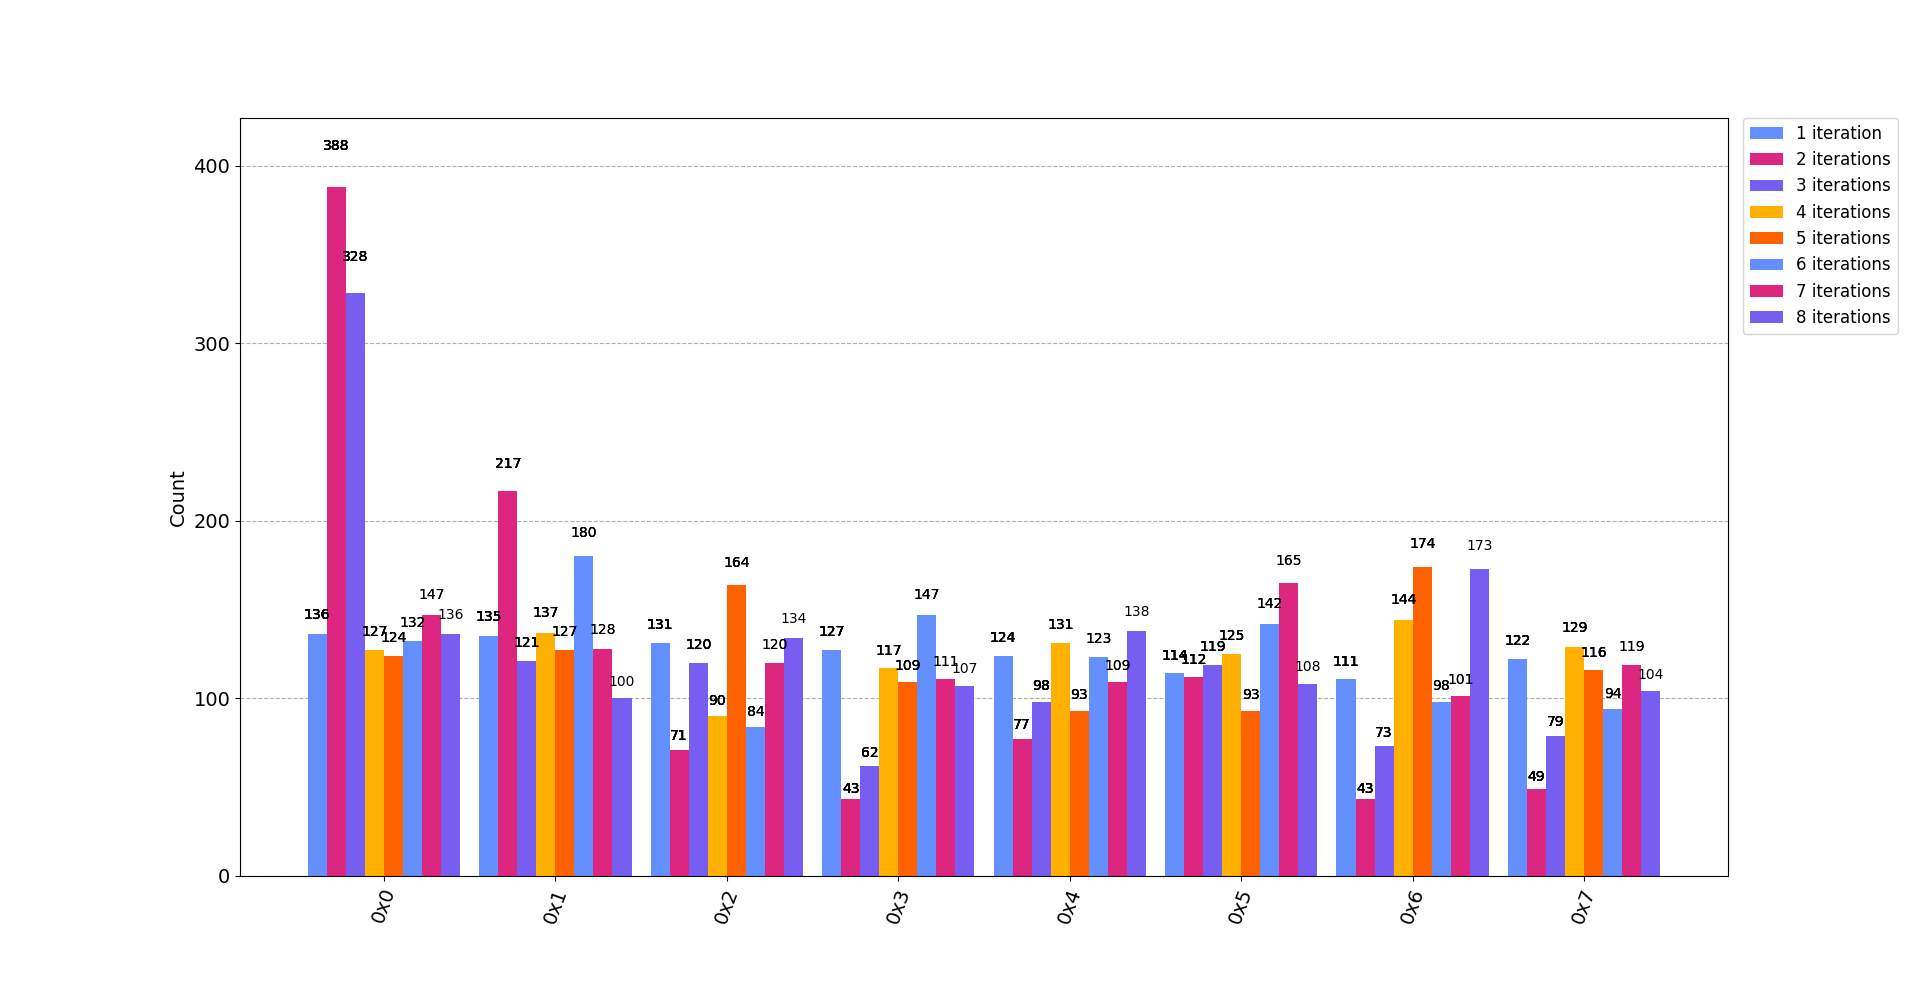
\includegraphics[width=\linewidth]{images/hardware/Figure_1_qc.png}
\end{figure}

It can be seen that the output is bit different with the real quantum computer than on the simulator, as the graph has now frequencies of different outcomes, rather than probabilities. However, the probabilities can be derived by dividing the frequency by the amount of all observations, which sums up to $1000$. It can be seen that at first with iterations $1 - 3$, the algorithm finds the correct result $\ket{000}$. At $4$ iterations and beyond, it gets the wrong result. In \ref{detailedgrover} it was stated that the algorithm should be in this case iterated $\frac{\pi}{4} \sqrt{2^{n}} = \frac{\pi}{4} \sqrt{8} = 2.22 $ times. It is clearly shown in the graph that the largest frequency, $388$ outcomes of $\ket{000}$, is achieved when the algorithm is iterated $2$ times. Therefore, the experiments some what correlates with the researched papers.

More detailed results of the job executed on the quantum computer can be found from Appendix \ref{appendix:testdataresults}.

\subsection{Comparing the results}
As stated in Chapter \ref{detailedgrover}, there is an optimal factor for the amount of iterations for the algorithm, and beyond that factor the results will become worse. This observation seems to be correct when the Grover's algorithm is run on the real quantum computer, as after $3$ iterations the algorithm gives wrong results. When run on the simulator, it only gave a wrong result once with $5$ iterations. Therefore, it seems that the simulator does not follow the results in the cited papers.

\chapter{Conclusion}
\label{chpater:conclusion}
%Summarize the research problem and the main contributions of previous papers. The main weakness of previous works could also be mentioned here. Some future works can be described as well.

Grover's algorithm is a quantum algorithm, which provides a quadratic speedup when searching unstructured databases using a quantum computer. Grover's algorithm is one of the well known and researched quantum algorithms, which development sped up the research in the field of quantum computing. Grover's algorithm has variations, as it can be used for partially searching a database instead of doing a full search. It has also applications outside of databases and data searching. Grover's algorithm can be applied to break encryption keys used in symmetric cryptographic schemes like AES, and to solve NP-complete problems, like the 3-SAT problem.

In this report, it was experimented how running Grover's algorithm on a simple search problem first in a simulator, and then on a real quantum computer differed. Conclusion was that the results gotten from the real quantum computer corresponded to the theoretical results in the papers cited on this report. It is shown that when the amount of iterations used in computing Grover's algorithm increases, the results get worse. However, in the simulator, when the iterations are increased, the gotten results do not show any change for the worse, excluding some individual ones. Therefore, it seems that the simulator does not obey the results in the researched papers.

Quantum computing is a new and emerging technology, which will have a significant influence to the field of computer science as we know it. If large enough and functioning quantum computers will be built, it would break the known public-key cryptography, which would have unfortunate consequenses. On the other hand however, the exponential computing power could possibly be used to solve some complex computing tasks, which would benefit various research fields. Most likely quantum computers will be used together with classical computers, in a hybrid manner. Same way as GPU's nowadays, quantum computers could be used to run only certain specific and  complex computing problems. There is not yet a lot of research in the field combining quantum computing and databases, but this might change in the future when the development of quantum computing and quantum computers goes forward.


% STEP 5: Uncomment the following lines and set your .bib file and
% desired bibliography style to make a bibliography with BibTeX.
% Alternatively you can use the thebibliography environment if you want
% to add all references by hand.
% 
\cleardoublepage %fixes the position of bibliography in bookmarks
\phantomsection

\renewcommand\bibname{References}
\addcontentsline{toc}{chapter}{\bibname} % This lines adds the bibliography to the ToC 
\bibliographystyle{abbrv} % numbering alphabetic order 
\bibliography{UH_DS_references}


\begin{appendices} 
\myappendixtitle

\chapter{Code used in running and analyzing Grover's algorithm} 
\label{appendix:code}

The code used in Section \ref{Allresults} related to running, experimenting and visualizing Grover's Algorithm can be found from my GitHub: \href{https://github.com/AlluSu/Quantum-Algorithms}{https://github.com/AlluSu/Quantum-Algorithms} 
\begin{verbatim}

\end{verbatim}

\chapter{Results of the test runs used in experimenting}
\label{appendix:testdataresults}
After each run, the results are saved in IBM's services where they can be viewed and analyzed later. The results from the experiments in Section \ref{Allresults} can be viewed in my GitHub:
\href{https://github.com/AlluSu/Quantum-Algorithms/tree/master/test-results/}{https://github.com/AlluSu/Quantum-Algorithms/tree/master/test-results/}

\end{appendices}
\end{document}
